\chapter{Τριγωνομετρία}
\section{Τριγωνομετρικοί αριθμοί}
\orismoi
\Orismos{Τριγωνομετρικοί αριθμοί}
Έστω $ AB\varGamma $ ένα ορθογώνιο τρίγωνο, με $ A=90\degree $ τότε οι τριγωνομετρικοί αριθμοί των οξειών γωνιών του τριγώνου ορίζονται ως εξής :\\
\begin{minipage}{\linewidth}\mbox{}\\
\vspace{-1cm}
\begin{WrapText1}{5}{3.3cm}
\vspace{-2mm}
\begin{tikzpicture}[scale=.8]
\tkzDefPoint(0,0){A}
\tkzDefPoint(3,0){B}
\tkzDefPoint(0,4){C}
\tkzMarkAngle[fill=\xrwma!50,size=.5](C,B,A)
\tkzMarkRightAngle[size=.3](B,A,C)
\tkzDrawPolygon[pl](A,B,C)
\tkzText(2.2,.2){$ \omega $}
\tkzLabelPoint[left](A){$ A $}
\tkzLabelPoint[right](B){$ B $}
\tkzLabelPoint[left](C){$ \varGamma $}
\tkzDrawPoints[size=7,fill=white](A,B,C)
\end{tikzpicture}\captionof{figure}{Τριγωνομετρικοί αριθμοί}
\end{WrapText1}
\begin{enumerate}[itemsep=0mm,label=\bf\arabic*.]
\item \textbf{Ημίτονο}\\
Ημίτονο μιας οξέιας γωνίας ενός ορθογωνίου τριγώνου ονομάζεται ο λόγος της απέναντι κάθετης πλευράς προς την υποτείνουσα.
\[ \textrm{Ημίτονο}=\frac{\textrm{Απέναντι Κάθετη}}{\textrm{Υποτείνουσα}}\;\;,\;\;\hm{\omega}=\frac{A\varGamma}{B\varGamma} \]
\item \textbf{Συνημίτονο}\\
Συνημίτονο μιας οξέιας γωνίας ενός ορθογωνίου τριγώνου ονομάζεται ο λόγος της προσκείμενης κάθετης πλευράς προς την υποτείνουσα.
\end{enumerate}
\[ \textrm{Συνημίτονο}=\frac{\textrm{Προσκείμενη Κάθετη}}{\textrm{Υποτείνουσα}}\;\;,\;\;\syn{\omega}=\frac{AB}{B\varGamma} \]
\begin{enumerate}[itemsep=0mm,label=\bf\arabic*.,start=3]
\item \textbf{Εφαπτομένη}\\
Εφαπτομένη μιας οξέιας γωνίας ενός ορθογωνίου τριγώνου ονομάζεται ο λόγος της απέναντι κάθετης πλευράς προς την προσκείμενη κάθετη.
\[ \textrm{Εφαπτομένη}=\frac{\textrm{Απέναντι Κάθετη}}{\textrm{Προσκείμενη Κάθετη}}\;\;,\;\;\ef{\omega}=\frac{A\varGamma}{AB} \]
\item \textbf{Συνεφαπτομένη}\\
Συνεφαπτομένη μιας οξέιας γωνίας ενός ορθογωνίου τριγώνου ονομάζεται ο λόγος της προσκείμενης κάθετης πλευράς προς την απέναντι κάθετη.
\[ \textrm{Συνεφαπτομένη}=\frac{\textrm{Προσκείμενη Κάθετη}}{\textrm{Απέναντι Κάθετη}}\;\;,\;\;\syf{\omega}=\frac{AB}{A\varGamma} \]
\end{enumerate}
\end{minipage}\mbox{}\\\\
Στον ακόλουθο πίνακα βλέπουμε τους τριγωνομετρικούς αριθμούς των βασικότερων γωνιών.
\begin{center}
\begin{tabular}{c||>{\centering\arraybackslash}m{.8cm}>{\centering\arraybackslash}m{.8cm}>{\centering\arraybackslash}m{.8cm}>{\centering\arraybackslash}m{.8cm}>{\centering\arraybackslash}m{.8cm}>{\centering\arraybackslash}m{.8cm}>{\centering\arraybackslash}m{.8cm}>{\centering\arraybackslash}m{.8cm}>{\centering\arraybackslash}m{.8cm}}
\hline  \multicolumn{10}{c}{\textbf{Βασικές Γωνίες}} \rule[-2ex]{0pt}{5.5ex}  \\ 
\hhline{==========} \rule[-2ex]{0pt}{5.5ex} \textbf{Μοίρες} & $ 0\degree $ & $ 30\degree $ & $ 45\degree $ & $ 60\degree $ & $ 90\degree $ & $ 120\degree $ & $ 135\degree $ & $ 150\degree $ & $ 180\degree $ \\ 
\rule[-2ex]{0pt}{4ex} \textbf{Ακτίνια} & $ 0 $ & $ \frac{\pi}{6} $ & $ \frac{\pi}{4} $ & $ \frac{\pi}{3} $ & $ \frac{\pi}{2} $ & $ \frac{2\pi}{3} $ & $ \frac{3\pi}{4} $ & $ \frac{5\pi}{6} $ & $ \pi $ \\ 
\hline \rule[-2ex]{0pt}{5.5ex} \textbf{Σχήμα} & \begin{tikzpicture}
\fill[fill=\xrwma!50] (0,0) -- (.3,0) arc (0:0:.3) -- cycle;
\draw (-.35,0) -- (.35,0);
\draw (0,-.35) -- (0,.35);
\draw (0,0) circle (.3);
\coordinate (A) at (0:.3);
\draw (0,0) -- (A);
\end{tikzpicture} & \begin{tikzpicture}
\fill[fill=\xrwma!50] (0,0) -- (.3,0) arc (0:30:.3) -- cycle;
\draw (-.35,0) -- (.35,0);
\draw (0,-.35) -- (0,.35);
\draw (0,0) circle (.3);
\coordinate (A) at (30:.3);
\draw (0,0) -- (A);
\end{tikzpicture} & \begin{tikzpicture}
\fill[fill=\xrwma!50] (0,0) -- (.3,0) arc (0:45:.3) -- cycle;
\draw (-.35,0) -- (.35,0);
\draw (0,-.35) -- (0,.35);
\draw (0,0) circle (.3);
\coordinate (A) at (45:.3);
\draw (0,0) -- (A);
\end{tikzpicture} & \begin{tikzpicture}
\fill[fill=\xrwma!50] (0,0) -- (.3,0) arc (0:60:.3) -- cycle;
\draw (-.35,0) -- (.35,0);
\draw (0,-.35) -- (0,.35);
\draw (0,0) circle (.3);
\coordinate (A) at (60:.3);
\draw (0,0) -- (A);
\end{tikzpicture} & \begin{tikzpicture}
\fill[fill=\xrwma!50] (0,0) -- (.3,0) arc (0:90:.3) -- cycle;
\draw (-.35,0) -- (.35,0);
\draw (0,-.35) -- (0,.35);
\draw (0,0) circle (.3);
\coordinate (A) at (90:.3);
\draw (0,0) -- (A);
\end{tikzpicture} & \begin{tikzpicture}
\fill[fill=\xrwma!50] (0,0) -- (.3,0) arc (0:120:.3) -- cycle;
\draw (-.35,0) -- (.35,0);
\draw (0,-.35) -- (0,.35);
\draw (0,0) circle (.3);
\coordinate (A) at (120:.3);
\draw (0,0) -- (A);
\end{tikzpicture} & \begin{tikzpicture}
\fill[fill=\xrwma!50] (0,0) -- (.3,0) arc (0:135:.3) -- cycle;
\draw (-.35,0) -- (.35,0);
\draw (0,-.35) -- (0,.35);
\draw (0,0) circle (.3);
\coordinate (A) at (135:.3);
\draw (0,0) -- (A);
\end{tikzpicture} & \begin{tikzpicture}
\fill[fill=\xrwma!50] (0,0) -- (.3,0) arc (0:150:.3) -- cycle;
\draw (-.35,0) -- (.35,0);
\draw (0,-.35) -- (0,.35);
\draw (0,0) circle (.3);
\coordinate (A) at (150:.3);
\draw (0,0) -- (A);
\end{tikzpicture} & \begin{tikzpicture}
\fill[fill=\xrwma!50] (0,0) -- (.3,0) arc (0:180:.3) -- cycle;
\draw (-.35,0) -- (.35,0);
\draw (0,-.35) -- (0,.35);
\draw (0,0) circle (.3);
\coordinate (A) at (180:.3);
\draw (0,0) -- (A);
\end{tikzpicture} \\ 
\hline \rule[-2ex]{0pt}{5ex} $ \hm{\omega} $ & $ 0 $ & $ \frac{1}{2} $ & $ \frac{\sqrt{2}}{2} $ & $ \frac{\sqrt{3}}{2} $ & $ 1 $ & $ \frac{\sqrt{3}}{2} $ & $ \frac{\sqrt{2}}{2} $ & $ \frac{1}{2} $ & $ 0 $ \\ 
\rule[-2ex]{0pt}{4ex} $ \syn{\omega} $ & $ 1 $ & $ \frac{\sqrt{3}}{2} $ & $ \frac{\sqrt{2}}{2} $ & $ \frac{1}{2} $ & $ 0 $ & $ -\frac{1}{2} $ & $ -\frac{\sqrt{2}}{2} $ & $ -\frac{\sqrt{3}}{2} $ & $ -1 $ \\ 
\rule[-2ex]{0pt}{4ex} $ \ef{\omega} $ & $ 0 $ & $ \frac{\sqrt{3}}{3} $ & $ 1 $ & $ \sqrt{3} $ & \begin{minipage}{.8cm}
\begin{center}
{\scriptsize Δεν\\\vspace{-1mm}ορίζεται}
\end{center}
\end{minipage} & $ -\sqrt{3} $ & $ -1 $ & $ -\frac{\sqrt{3}}{3} $ & $ 0 $ \\
\rule[-2ex]{0pt}{4ex} $ \syf{\omega} $ & \begin{minipage}{.8cm}
\begin{center}
{\scriptsize Δεν\\\vspace{-1mm}ορίζεται}
\end{center}
\end{minipage} & $ \sqrt{3} $ & $ 1 $ & $ \frac{\sqrt{3}}{3} $ & $ 0 $ & $ -\frac{\sqrt{3}}{3} $ & $ -1 $ & $ -\sqrt{3} $ & \begin{minipage}{.8cm}
\begin{center}
{\scriptsize Δεν\\\vspace{-1mm}ορίζεται}
\end{center}
\end{minipage} \\ 
\hline 
\end{tabular}\captionof{table}{Τριγωνομετρικοί αριθμοί βασικών γωνιών}
\end{center}\mbox{}\\
\Orismos{τριγωνομετρικοσ κυκλοσ}
Τριγωνομετρικός κύκλος ονομάζεται ο κύκλος με ακτίνα  και κέντρο την αρχή των αξόνων ενός ορθογωνίου συστήματος συντεταγμένων, στους άξονες του οποίου παίρνουν τιμές οι τριγωνομετρικοί αριθμοί των γωνιών.
\begin{center}
\begin{tabular}{p{6.85cm}p{6.85cm}}
\begin{tikzpicture}[>=latex,scale=2]
\fill[fill=black!50] (0,0) -- (.2,0) arc (0:60:.2) -- cycle;
%axis
\draw[->] (-1.2,0) -- coordinate (x axis mid) (1.5,0) node[right,fill=white] {{\footnotesize $ x $}};
\foreach \x in {-1,-0.8,-0.6,-0.4,-0.2,0,0.2,0.4,0.6,0.8,1}
\draw (\x,.5pt) -- (\x,-.5pt)
node[anchor=north] {{\tiny \x}};
\foreach \y in {-1,-0.8,-0.6,-0.4,-0.2,0,0.2,0.4,0.6,0.8,1}
\draw (.5pt,\y) -- (-.5pt,\y)
node[anchor=east] {{\tiny \y}};
\draw[->] (0,-1.2) -- (0,1.5) node[above,fill=white] {{\footnotesize $ y $}};
\draw[-] (1,-1.2) -- (1,1.8);
\draw[-] (-1.2,1) -- (1.2,1);
\draw[-,thick] (0,1) -- (1.732/3,1);
\draw[-,thick] (1,0) -- (1,1.732);
\draw[-,dashed] (-.7,-1.732*0.7) -- (1,1.732);
\draw circle (1);
\coordinate (A) at (60:1);
\tkzDefPoint(0,0){O}
\tkzDefPoint(cos(pi/3),0){B}
\tkzDefPoint(0,sin(pi/3)){C}
\tkzDefPoint(1,tan(pi/3)){D}
\tkzDefPoint(cot(pi/3),1){E}
\tkzDefPoint(1,0){F}
\tkzDefPoint(0,1){G}
\tkzDrawSegment(O,A)
\tkzDrawSegments[thin,dashed](A,B A,C)
\tkzText(0,1.75){{\scriptsize Άξονας Ημιτόνων}}
\tkzText(1.6,-.12){{\scriptsize Άξονας}}
\tkzText(1.6,-.23){{\scriptsize Συνημιτόνων}}
\tkzText(-1,1.2){{\scriptsize Άξονας}}
\tkzText(-.75,1.1){{\scriptsize Συνεφαπτομένων}}
\tkzText(1.23,-.9){{\scriptsize Άξονας}}
\tkzText(1.4,-1){{\scriptsize Εφαπτομένων}}
\tkzText(-.5,-1.1){{\scriptsize $ \delta $}}
\tkzDrawSegment[thick](O,B)
\tkzDrawSegment[thick](O,C)
\tkzDrawPoints[size=7,fill=white](O,A,B,C,D,E,F,G)
\tkzText(-.4,.43){{{\scriptsize \textrm{ημ}$ \omega $}}$\LEFTRIGHT\{.{ \rule{0pt}{18mm} } $}
\tkzText(.25,-.25){$ \undercbrace{\rule{9mm}{0mm}}_{{\scriptsize \textrm{συν}\omega}} $}
\tkzText(1.2,.87){$\LEFTRIGHT.\}{ \rule{0pt}{35mm} } ${{\scriptsize \textrm{εφ}$ \omega $}}}
\tkzText(.3,1.12){$ \overcbrace{\rule{11mm}{0mm}}^{{\scriptsize \textrm{σφ}\omega}} $}
\tkzText(.25,.15){$ \omega $}
\tkzLabelPoint[below left](O){{\tiny $ O $}}
\tkzLabelPoint[above=1mm,right](A){{\tiny $ M $}}
\tkzLabelPoint[above right](B){{\tiny $ M_1 $}}
\tkzLabelPoint[above=1mm, left](C){{\tiny $ M_2 $}}
\tkzLabelPoint[left](D){{\tiny $ K $}}
\tkzLabelPoint[above](E){{\tiny $ \varLambda $}}
\tkzLabelPoint[below right](F){{\tiny $ A $}}
\tkzLabelPoint[above left](G){{\tiny $ B $}}
\draw [->] (.984*.9,.173*.9) arc (10:45:.9);
\draw [->] (.984*.9,-.173*.9) arc (-10:-45:.9);
\tkzText(.72,.35){$ + $}
\tkzText(.72,-.35){$ - $}
\tkzText(.35,.45){$ \rho $}
\tkzText(-1,.9){{\scriptsize $ \varepsilon_2 $}}
\tkzText(.9,-1){{\scriptsize $ \varepsilon_1 $}}
\end{tikzpicture}\captionof{figure}{Τριγωνομετρικός κύκλος} & 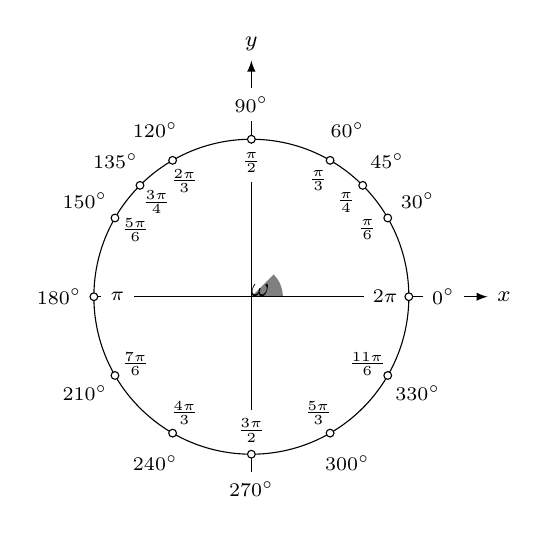
\begin{tikzpicture}[>=latex,scale=2]
\fill[fill=black!50] (0,0) -- (.2,0) arc (0:45:.2) -- cycle;
%axis
\draw[->] (-1.2,0) -- (1.5,0) node[right,fill=white] {{\footnotesize $ x $}};
\draw[->] (0,-1.2) -- (0,1.5) node[above,fill=white] {{\footnotesize $ y $}};

\foreach \gwnia/\xtext in {
30/\frac{\pi}{6},
45/\frac{\pi}{4},
60/\frac{\pi}{3},
90/\frac{\pi}{2},
120/\frac{2\pi}{3},
135/\frac{3\pi}{4},
150/\frac{5\pi}{6},
180/\pi,
210/\frac{7\pi}{6},
240/\frac{4\pi}{3},
270/\frac{3\pi}{2},
300/\frac{5\pi}{3},
330/\frac{11\pi}{6},
360/2\pi}
\draw (\gwnia:0.85cm) node {{\scriptsize $\xtext$}};
\foreach \gwnia/\xtext in {
90/\frac{\pi}{2},
180/\pi,
270/\frac{3\pi}{2},
360/2\pi}
\draw (\gwnia:0.85cm) node[fill=white] {{\scriptsize $\xtext$}};
\tkzDefPoint(0,0){O}
\coordinate (A) at (45:1);
\tkzDrawSegment(O,A)
\draw circle (1);
\foreach \gwnia in {0,30,45,60,90,120,135,150,180,210,240,270,300,330}{
\coordinate (P) at (\gwnia:1);
\draw (\gwnia:1.22cm) node[fill=white] {{\scriptsize $\gwnia^\circ$}};
\draw[draw=black,fill=white] (P) circle (.7pt);};
\tkzText(.25,.1){$ \omega $}
\end{tikzpicture}\captionof{figure}{Βασικές γωνίες}
\end{tabular}
\end{center}
\begin{itemize}[itemsep=0mm]
\item Κάθε γωνία $ \omega $ έχει πλευρές, τον θετικό ημιάξονα $ Ox $ και την ακτίνα $ \rho $ του κύκλου, μετρώντας τη γωνία αυτή αριστερόστροφα, φορά που ορίζεται ως \textbf{θετική}.
\item Ο οριζόντιος άξονας $ x'x $ είναι ο άξονας συνημιτόνων ενώ ο κατακόρυφος $ y'y $ ο άξονας ημιτόνων.
\item Κάθε σημείο $ M $ του κύκλου έχει συντεταγμένες $ M(\syn{\omega},\hm{\omega}) $.
\item Η τετμημέμη του σημείου είναι ίση με το συνημίτονο της γωνίας, ενώ η τεταγμένη ίση με το ημίτονο της.
\[ x=\syn{\omega}\;\;,\;\;y=\hm{\omega} \]
\item Η εφαπτόμενη ευθεία στον κύκλο στο σημείο $ A(1,0) $ είναι ο \textbf{άξονας των εφαπτομένων}. Η εφαπτομένη της γωνίας $ \omega $ είναι η τεταγμένη του σημείου τομής της ευθείας $ \varepsilon_1 $ με το φορέα $ \delta $ της ακτίνας.
\[ y_{\!_K}=\ef{\omega} \]
\item Η εφαπτόμενη ευθεία στον κύκλο στο σημείο $ B(0,1) $ είναι ο \textbf{άξονας των συνεφαπτομένων}. Η συνεφαπτομένη της γωνίας $ \omega $ είναι η τετμημένη του σημείου τομής της ευθείας $ \varepsilon_2 $ με το φορέα $ \delta $ της ακτίνας.
\[ x_{\!_K}=\syf{\omega} \]	
\end{itemize}
\Orismos{τριγ. αρ. γωνιασ σε συστημα συντεταγμενων}
Έστω $ Oxy $ ένα ορθογώνιο σύστημα συντεταγμένων και $ M(x,y) $ ένα σημείο του. Ενώνοντας το σημείο $ M $ με την αρχή των αξόνων, το ευθύγραμμο τμήμα που προκύπτει δημιουργεί μια γωνία $ \omega $ με το θετικό οριζόντιο ημιάξονα $ Ox $.
Το μήκος του ευθύγραμμου τμήματος $ OM $ είναι :
\[ OM=\rho=\sqrt{x^2+y^2} \]
Οι τριγωνομετρικοί αριθμοί της γωνίας αυτής ορίζονται με τη βοήθεια των συντεταγμένων του σημείου και είναι :\\
\begin{minipage}{\linewidth}\mbox{}\\
\vspace{-1cm}
\begin{WrapText1}{14}{4.7cm}
\vspace{.5cm}
\begin{tikzpicture}[y=.8cm,x=.9cm]
\draw[draw=black,fill=black!10] (0,0) -- (.5,0) arc (0:40:.5) -- cycle;
\draw[-latex]  (-.4,0)  -- coordinate (x axis mid) (4,0) node[right,fill=white] {{\footnotesize $ x $}};
\draw[-latex] (0,-.4) -- (0,3.5) node[above,fill=white] {{\footnotesize $ y $}};
\draw (3,.1) -- (3,-.1) node[anchor=north] {\scriptsize $ x $};
\draw (.1,2.5) -- (-.1,2.5) node[anchor=east] {\scriptsize $ y $};
\draw[dashed] (3,0) -- (3,2.5) -- (0,2.5);
\tkzDefPoint(0,0){O}
\tkzDefPoint(3,2.5){M}
\tkzDefPoint(3,0){A}
\tkzDefPoint(0,2.5){B}
\tkzDrawSegment(O,M)
\tkzDrawPoint[size=7,fill=white](M)
\tkzDrawPoint[size=7,fill=white](A)
\tkzDrawPoint[size=7,fill=white](B)
\tkzLabelPoint[below left](O){$ O $}
\tkzLabelPoint[above](M){$ M(x,y) $}
\tkzLabelPoint[above right](A){{\footnotesize $ A(x,0) $}}
\tkzLabelPoint[above right](B){{\footnotesize $ B(0,y) $}}
\tkzText(1.5,-.4){$ \undercbrace{\rule{25mm}{0mm}}_{{\scriptsize x}} $}
\tkzText(-.3,1.25){{{\scriptsize $ y $}}$\LEFTRIGHT\{.{ \rule{0pt}{20mm} } $}
\tkzText[fill=white,inner sep=.2mm](2.7,1){{\footnotesize $ \rho=\sqrt{x^2+y^2} $}}
\tkzText(.7,.2){{\footnotesize $ \omega $}}
\end{tikzpicture}\captionof{figure}{Τριγωνομετρικοί αριθμοί σε σύστημα συντεταγμένων}\end{WrapText1}
\begin{enumerate}[itemsep=0mm,label=\bf\arabic*.]
\item \textbf{Ημίτονο}\\
Ημίτονο της γωνίας $ \omega $ ονομάζεται ο λόγος της τεταγμένης του σημείου προς την απόσταση του από την αρχή των αξόνων.
\[ \hm{\omega}=\frac{AM}{OM}=\frac{y}{\rho} \]
\item \textbf{Συνημίτονο}\\
Συνημίτονο της γωνίας $ \omega $ ονομάζεται ο λόγος της τετμημένης του σημείου προς την απόσταση του από την αρχή των αξόνων.
\[ \syn{\omega}=\frac{BM}{OM}=\frac{x}{\rho} \]
\end{enumerate}

\begin{enumerate}[itemsep=0mm,label=\bf\arabic*.,start=3]
\item \textbf{Εφαπτομένη}\\
Εφαπτομένη της γωνίας $ \omega $ τριγώνου ονομάζεται ο λόγος της τεταγμένης του σημείου προς την τετμημένη του.
\[ \ef{\omega}=\frac{AM}{BM}=\frac{y}{x}\;\;,\;\;x\neq0 \]
\item \textbf{Συνεφαπτομένη}\\
Συνεφαπτομένη της γωνίας $ \omega $ ονομάζεται ο λόγος της τετμημένης του σημείου προς την τεταγμένη του.
\[ \syf{\omega}=\frac{BM}{AM}=\frac{x}{y}\;\;.\;\;y\neq0 \]
\end{enumerate}\end{minipage}\mbox{}\\\\\\
\thewrhmata
\Thewrhma{Άκρα τριγωνομετρικών αριθμών}
To ημίτονο και το συνημίτονο οποιασδήποτε γωνίας $ \omega $ παίρνει τιμές από $-1$ μέχρι $ 1 $. Οι παρακάτω σχέσεις είναι ισοδύναμες :
\begin{multicols}{2}
\begin{rlist}
\item  $ -1\leq\hm{\omega}\leq1\;\;,\;\;-1\leq\syn{\omega}\leq1 $
\item $ |\hm{\omega}|\leq1\ ,\ |\syn{\omega}|\leq1 $
\end{rlist}
\end{multicols}
\Thewrhma{βασικεσ τριγωνομετρικεσ ταυτοτητεσ}
Για οποιαδήποτε γωνία $ \omega $ ισχύουν οι παρακάτω βασικές τριγωνομετρικές ταυτότητες :
\begin{multicols}{3}
\begin{enumerate}[itemsep=0mm]
\item $ \hm^2{\omega}+\syn^2{\omega}=1 $
\item $ \ef{\omega}={\dfrac{\hm{\omega}}{\syn{\omega}}} $
\item $ \syf{\omega}={\dfrac{\syn{\omega}}{\hm{\omega}}} $
\item $ \ef{\omega}\cdot\syf{\omega}=1 $
\item $ \syn^2{\omega}=\dfrac{1}{1+\ef^2{\omega}} $
\item $ \hm^2{\omega}=\dfrac{\ef^2{\omega}}{1+\ef^2{\omega}} $
\end{enumerate}
\end{multicols}
\Thewrhma{αναγωγη στο 1\textsuperscript{\MakeLowercase{o}} τεταρτημοριο}\label{th:an_tet}
Οι τριγωνομετρικοί αριθμοί γωνιών που καταλήγουν στο 2\tss{ο}, 3\tss{ο} ή 4\tss{ο} ανάγωνται σε τριγωνομετρικούς αριθμούς γωνιών του 1\textsuperscript{ου} τεταρτημορίου σύμφωνα με τους παρακάτω τύπους.
\begin{enumerate}[itemsep=0mm,label=\bf\arabic*.]
\item \textbf{Παραπληρωματικές γωνίες (2\textsuperscript{ο} τεταρτημόριο)}\\
Γωνίες που καταλήγουν στο 2\tss{ο} τεταρτημόριο μπορούν να γραφτούν ως παραπληρωματικές γωνιών του 1\tss{ου} τεταρτημορίου. Εαν $ \omega $ είναι μια γωνία του 1\textsuperscript{ου} τεταρτημορίου τότε η παραπληρωματική της θα είναι της μορφής $ 180\degree-\omega $. Οι σχέσεις μεταξύ των τριγωνομετρικών τους αριθμών φαίνονται παρακάτω :\\
\begin{minipage}{\linewidth}\mbox{}\\
\vspace{-1cm}
\begin{WrapText1}{7}{6cm}
\begin{tikzpicture}[>=latex,scale=2]
\clip (-1.5,-.3) rectangle (1.4,1.4);
\draw[fill=\xrwma!10] (0,0) -- (.2,0) arc (0:40:.2) -- cycle;
\draw[fill=\xrwma!30] (0,0) -- (.15,0) arc (0:140:.15) -- cycle;
%axis
\draw[->] (-1.2,0) -- (1.2,0) node[right,fill=white] {{\footnotesize $ x $}};
\draw[->] (0,-1.2) -- (0,1.2) node[above,fill=white] {{\footnotesize $ y $}};
\tkzDefPoint(0,0){O}
\tkzDefPoint(cos(2*pi/9),0){D}
\tkzDefPoint(-cos(2*pi/9),0){E}
\tkzDefPoint(0,sin(2*pi/9)){F}
\coordinate (A) at (40:1);
\coordinate (B) at (140:1);
\tkzDrawSegments(O,A O,B)
\draw circle (1);
\tkzText(.3,.1){{\footnotesize $ \omega $}}

\tkzText(0,.3){{\footnotesize $ 180^{\mathrm{o}}-\omega $}}
\draw[dashed] (A) -- (D) node[anchor=north]{{\footnotesize $ x $}};
\draw[dashed] (B) -- (E)node[anchor=north]{{\footnotesize $ -x $}};
\draw[dashed] (A) -- (B);
\tkzDrawPoints[size=7,fill=white](A,B,D,E,F)
\tkzLabelPoint[above left](F){{\footnotesize $ y $}}
\tkzLabelPoint[above right](A){{\footnotesize $ M(x,y) $}}
\tkzLabelPoint[above left](B){{\footnotesize $ N(-x,y) $}}
\tkzLabelPoint[below left](O){$ O $}
\end{tikzpicture}
\end{WrapText1}
\begin{itemize}[itemsep=0mm]
\item $ \hm{\left( 180\degree-\omega\right) }=\hm{\omega} $
\item $ \syn{\left( 180\degree-\omega\right) }=-\syn{\omega} $
\item $ \ef{\left( 180\degree-\omega\right) }=-\ef{\omega} $
\item $ \syf{\left( 180\degree-\omega\right) }=-\syf{\omega} $
\end{itemize}
Οι παραπληρωματικές γωνίες έχουν ίσα ημίτονα και αντίθετους όλους τους υπόλοιπους τριγωνομετρικούς αριθμούς. Τα σημεία $ M,N $ του τριγωνομετρικού κύκλου, των γωνιών $ \omega $ και $ 180\degree-\omega $ αντίστοιχα, είναι συμμετρικα ως προς άξονα $ y'y $ και κατά συνέπεια έχουν αντίθετες τετμημένες.
\end{minipage}
\item \textbf{Γωνίες με διαφορά $ \mathbold{180\degree} $ (3\tss{ο} Τεταρτημόριο)}\\
Γωνίες που καταλήγουν στο 3\tss{ο} τεταρτημόριο μπορούν να γραφτούν ως γωνίες με διαφορά $ 180\degree $ γωνιών του 1\tss{ου} τεταρτημορίου. Εάν $ \omega $ είναι μια γωνία του 1\textsuperscript{ου} τεταρτημορίου, η γωνία η οποία διαφέρει από την $ \omega $ κατά $ 180\degree $ θα είναι της μορφής $ 180\degree+\omega $. Οι σχέσεις που συνδέουν τους τριγωνομετρικούς αριθμούς των δύο γωνιών θα είναι :\\
\begin{minipage}{\linewidth}\mbox{}\\
\vspace{-1cm}
\begin{WrapText2}{12}{4cm}
\begin{tikzpicture}[>=latex,scale=1.5]
\draw[fill=\xrwma!10] (0,0) -- (.2,0) arc (0:40:.2) -- cycle;
\draw[fill=\xrwma!30] (0,0) -- (.15,0) arc (0:220:.15) -- cycle;
%axis
\draw[->] (-1.2,0) -- (1.2,0) node[right,fill=white] {{\footnotesize $ x $}};
\draw[->] (0,-1.2) -- (0,1.2) node[above,fill=white] {{\footnotesize $ y $}};
\tkzDefPoint(0,0){O}
\tkzDefPoint(cos(2*pi/9),0){D}
\tkzDefPoint(-cos(2*pi/9),0){E}
\tkzDefPoint(0,-sin(2*pi/9)){F}
\tkzDefPoint(0,sin(2*pi/9)){C}
\coordinate (A) at (40:1);
\coordinate (B) at (220:1);
\tkzDrawSegments(O,A O,B)
\draw circle (1);
\tkzText(.3,.1){{\footnotesize $ \omega $}}

\tkzText(-.2,.27){{\footnotesize $ 180^{\mathrm{o}}+\omega $}}
\draw[dashed] (A) -- (D) node[anchor=north]{{\footnotesize $ x $}};
\draw[dashed] (B) -- (E)node[anchor=south]{{\footnotesize $ -x $}};
\draw[dashed] (A) -- (C);
\draw[dashed] (B) -- (F);
\tkzDrawPoints[size=7,fill=white](A,B,C,D,E,F)
\tkzLabelPoint[left](C){{\footnotesize $ y $}}
\tkzLabelPoint[right](F){{\footnotesize $ -y $}}
\tkzLabelPoint[above,fill=white,inner sep=.2mm,yshift=1mm](A){{\footnotesize $ M(x,y) $}}
\tkzLabelPoint[below,fill=white,inner sep=.2mm,yshift=-1mm](B){{\footnotesize $ N(-x,-y) $}}
\tkzLabelPoint[below right](O){$ O $}
\end{tikzpicture}
\end{WrapText2}
\begin{multicols}{2}
\begin{itemize}[itemsep=0mm,leftmargin=2mm]
\item $ \hm{\left( 180\degree+\omega\right) }=-\hm{\omega} $
\item $ \syn{\left( 180\degree+\omega\right) }=-\syn{\omega} $
\item $ \ef{\left( 180\degree+\omega\right) }=\ef{\omega} $
\item $ \syf{\left( 180\degree+\omega\right) }=\syf{\omega} $
\end{itemize}
\end{multicols}
Οι γωνίες με διαφορά $ 180\degree $ έχουν αντίθετα ημίτονα και συνημίτονα ενώ έχουν ίσες εφαπτομένες και συνεφαπτομένες. Τα σημεία $ M,N $ του τριγωνομετρικού κύκλου, των γωνιών $ \omega $ και $ 180\degree+\omega $ αντίστοιχα, είναι συμμετρικά ως προς την αρχή των αξόνων και κατά συνέπεια έχουν αντίθετες συντεταγμένες.
\end{minipage}
\item \textbf{Αντίθετες γωνίες - Γωνίες με άθροισμα {\boldmath{$ 360\degree $}} (4\textsuperscript{ο} Τεταρτημόριο)}\\
Γωνίες που καταλήγουν στο 4\tss{ο} τεταρτημόριο μπορούν να γραφτούν ως αντίθετες γωνιών του 1\tss{ου} τεταρτημορίου. Η αντίθετη γωνία, μιας γωνίας $ \omega $ του 1\textsuperscript{ου} τεταρτημορίου, ορίζεται να είναι η γωνία η οποία έχει ίσο μέτρο με τη γωνία $ \omega $, με φορά αντίθετη απ' αυτήν και θα έχει τη μορφή $ -\omega $. Επιπλέον η γωνία η οποία έχει με τη γωνία $ \omega $, άθροισμα $ 360\degree $ καταλήγει στο ίδιο σημείο και θα είναι $ 360\degree-\omega $.\\
\begin{minipage}{\linewidth}\mbox{}\\
\vspace{-1cm}
\begin{WrapText1}{9}{4.3cm}
\begin{tikzpicture}[>=latex,scale=1.5]
\draw[fill=\xrwma!10] (0,0) -- (.2,0) arc (0:40:.2) -- cycle;
\draw[fill=\xrwma!30] (0,0) -- (.15,0) arc (0:320:.15) -- cycle;
\draw[fill=\xrwma!50] (0,0) -- (.25,0) arc (0:-40:.25) -- cycle;
%axis
\draw[->] (-1.2,0) -- (1.2,0) node[right,fill=white] {{\footnotesize $ x $}};
\draw[->] (0,-1.2) -- (0,1.2) node[above,fill=white] {{\footnotesize $ y $}};
\tkzDefPoint(0,0){O}
\tkzDefPoint(cos(2*pi/9),0){D}
\tkzDefPoint(0,-sin(2*pi/9)){F}
\tkzDefPoint(0,sin(2*pi/9)){C}
\coordinate (A) at (40:1);
\coordinate (B) at (320:1);
\tkzDrawSegments(O,A O,B)
\draw circle (1);
\tkzText(.3,.1){{\footnotesize $ \omega $}}
\tkzText(.35,-.1){{\footnotesize $ -\omega $}}
\tkzText(-.2,.27){{\footnotesize $ 360^{\mathrm{o}}-\omega $}}
\draw[dashed] (A) -- (B);
\draw[dashed] (B) -- (F);
\draw[dashed] (A) -- (C);
\tkzDrawPoints[size=7,fill=white](A,B,C,D,F)
\tkzLabelPoint[left](C){{\footnotesize $ y $}}
\tkzLabelPoint[left](F){{\footnotesize $ -y $}}
\tkzLabelPoint[above right](A){{\footnotesize $ M(x,y) $}}
\tkzLabelPoint[below right](B){{\footnotesize $ N(x,-y) $}}
\tkzLabelPoint[below left](O){$ O $}
\end{tikzpicture}
\end{WrapText1}
\begin{itemize}[itemsep=0mm]
\item $ \hm{\left( -\omega\right) }=\hm{\left( 360\degree-\omega\right) }=-\hm{\omega} $
\item $ \syn{\left( -\omega\right) }=\syn{\left( 360\degree-\omega\right) }=\syn{\omega} $
\item $ \ef{\left( -\omega\right) }=\ef{\left( 360\degree-\omega\right) }=-\ef{\omega} $
\item $ \syf{\left( -\omega\right) }=\syf{\left( 360\degree-\omega\right) }=-\syf{\omega} $
\end{itemize}
Οι γωνίες με άθροισμα $ 360\degree $ καθώς και οι αντίθετες έχουν ίσα συνημίτονα και αντίθετους όλους τους υπόλοιπους τριγωνομετρικούς αριθμούς. Τα σημεία $ M,N $ του τριγωνομετρικού κύκλου, των γωνιών $ \omega $ και $ 360\degree-\omega $ αντίστοιχα, είναι συμμετρικα ως προς τον άξονα $ x'x $ και κατά συνέπεια έχουν αντίθετες τεταγμένες. Τα σημεία του κύκλου των γωνιών $ 360\degree-\omega $ και $ -\omega $ καθώς και οι ακτίνες τους ταυτίζονται.
\end{minipage}
\item \textbf{Συμπληρωματικές γωνίες}\\
Η συμπληρωματική γωνία μιας οξείας γωνίας $ \omega $ θα είναι της μορφής $ 90\degree-\omega $ η οποία ανήκει και αυτή στο 1\textsuperscript{ο} τεταρτημόριο. Οι τριγωνομετρικοί αριθμοί τους συνδέονται από τις παρακάτω σχέσεις :\\
\begin{minipage}{\linewidth}\mbox{}\\
\vspace{-1cm}
\begin{WrapText2}{13}{5cm}
\begin{tikzpicture}[>=latex,scale=2.5]
\clip (-.35,-.3) rectangle (1.4,1.4);
\draw[fill=\xrwma!10] (0,0) -- (.2,0) arc (0:30:.2) -- cycle;
\draw[fill=\xrwma!30] (0,0) -- (.15,0) arc (0:60:.15) -- cycle;
%axis
\draw[->] (-1.2,0) -- (1.2,0) node[right,fill=white] {{\footnotesize $ x $}};
\draw[->] (0,-1.2) -- (0,1.2) node[above,fill=white] {{\footnotesize $ y $}};
\tkzDefPoint(0,0){O}
\tkzDefPoint(cos(pi/6),0){D}
\tkzDefPoint(0,sin(pi/6)){C}
\tkzDefPoint(cos(pi/3),0){E}
\tkzDefPoint(0,sin(pi/3)){F}
\coordinate (A) at (30:1);
\coordinate (B) at (60:1);
\tkzDrawSegments(O,A O,B)
\draw circle (1);
\tkzText(.3,.07){{\footnotesize $ \omega $}}
\tkzText(-.1,.27){{\footnotesize $ 90^{\mathrm{o}}-\omega $}}
\draw[dashed] (A) -- (B);
\draw[dashed] (B) -- (F);
\draw[dashed] (B) -- (E);
\draw[dashed] (A) -- (C);
\draw[dashed] (A) -- (D);
\draw (-.3,-.3) -- (.8,.8);
\draw[-latex] (-.1,.23) -- (0.12,0.02);
\tkzDrawPoints[size=7,fill=white](A,B,C,D,E,F)
\tkzLabelPoint[left](C){{\footnotesize $ y_{\!_M} $}}
\tkzLabelPoint[below](D){{\footnotesize $ x_{\!_M} $}}
\tkzLabelPoint[left](F){{\footnotesize $ y_{\!_N} $}}
\tkzLabelPoint[below](E){{\footnotesize $ x_{\!_N} $}}
\tkzLabelPoint[above right](A){{\footnotesize $ M(x,y) $}}
\tkzLabelPoint[above right](B){{\footnotesize $ N(y,x) $}}
\tkzLabelPoint[below left](O){$ O $}
\tkzText(1,.75){{\footnotesize $ y=x $}}
\end{tikzpicture}
\end{WrapText2}
\begin{multicols}{2}
\begin{itemize}[itemsep=0mm,leftmargin=3mm]
\item $ \hm{\left( 90\degree-\omega\right) }=\syn{\omega} $
\item $ \syn{\left( 90\degree-\omega\right) }=\hm{\omega} $
\item $ \ef{\left( 90\degree-\omega\right) }=\syf{\omega} $
\item $ \syf{\left( 90\degree-\omega\right) }=\ef{\omega} $
\end{itemize}
\end{multicols}
Για δύο συμπληρωματικές γωνίες έχουμε οτι το ημίτονο της μιας είναι ίσο με το συνημίτονο της άλλης και η εφαπτομένη της μιας είναι ίση με τη συνεφαπτομένη της άλλης. Τα σημεία $ M,N $ του τριγωνομετρικού κύκλου, των γωνιών $ \omega $ και $ 90\degree-\omega $ αντίστοιχα, είναι συμμετρικα ως προς την ευθεία $ y=x $ οπότε έχουν συμμετρικές συντεταγμένες.
\end{minipage}
\item \textbf{Γωνίες με διαφορά $ \mathbold{90\degree} $}\\
\begin{minipage}{\linewidth}\mbox{}\\
\vspace{-5mm}
\begin{WrapText1}{9}{4.7cm}
\begin{tikzpicture}[>=latex,scale=1.8]
\clip (-1.25,-.3) rectangle (1.5,1.4);
\draw[fill=\xrwma!30] (0,0) -- (.2,0) arc (0:30:.2) -- cycle;
\draw[fill=\xrwma!50] (0,0) -- (.15,0) arc (0:120:.15) -- cycle;
%axis
\draw[->] (-1.2,0) -- (1.2,0) node[right,fill=white] {{\footnotesize $ x $}};
\draw[->] (0,-1.2) -- (0,1.2) node[above,fill=white] {{\footnotesize $ y $}};
\tkzDefPoint(0,0){O}
\tkzDefPoint(cos(pi/6),0){D}
\tkzDefPoint(0,sin(pi/6)){C}
\tkzDefPoint(cos(2*pi/3),0){E}
\tkzDefPoint(0,sin(2*pi/3)){F}
\coordinate (A) at (30:1);
\coordinate (B) at (120:1);
\tkzDrawSegments(O,A O,B)
\draw circle (1);
\tkzText(.3,.07){{\footnotesize $ \omega $}}
\tkzText(0.17,.27){{\footnotesize $ 90^{\mathrm{o}}+\omega $}}
\draw[dashed] (B) -- (F);
\draw[dashed] (B) -- (E);
\draw[dashed] (A) -- (C);
\draw[dashed] (A) -- (D);
\draw[->] (0.16,0.22) -- (0.04,0.06);
\tkzDrawPoints[size=7,fill=white](A,B,C,D,E,F)
\tkzLabelPoint[left](C){{\footnotesize $ y_{\!_M} $}}
\tkzLabelPoint[below](D){{\footnotesize $ x_{\!_M} $}}
\tkzLabelPoint[right](F){{\footnotesize $ y_{\!_N} $}}
\tkzLabelPoint[below](E){{\footnotesize $ x_{\!_N} $}}
\tkzLabelPoint[above right,xshift=-2mm,fill=white,inner sep=.2mm,yshift=2mm](A){{\footnotesize $ M(x,y) $}}
\tkzLabelPoint[above left](B){{\footnotesize $ N(-y,x) $}}
\tkzLabelPoint[below left](O){$ O $}
\tkzMarkRightAngle[size=.08](A,O,B)
\end{tikzpicture}
\end{WrapText1}
Γωνίες οι οποίες διαφέρουν κατά $ 90\degree $ έχουν τη μορφή $ \omega $ και $ 90\degree+\omega $. Οι τριγωνομετρικοί αριθμοί της γωνίας $ 90\degree+\omega $ δίνονται από τις παρακάτω σχέσεις :
\begin{multicols}{2}
\begin{itemize}[itemsep=0mm,leftmargin=2mm]
\item $ \hm{\left( 90\degree+\omega\right) }=\syn{\omega} $
\item $ \syn{\left( 90\degree+\omega\right) }=-\hm{\omega} $
\item $ \ef{\left( 90\degree+\omega\right) }=-\syf{\omega} $
\item $ \syf{\left( 90\degree+\omega\right) }=-\ef{\omega} $
\end{itemize}
\end{multicols}
Για δύο γωνίες με διαφορά $ 90\degree $ ισχύει οτι το ημίτονο της μιας είναι ίσο με το συνημίτονο της άλλης, ενώ συνημίτονο, εφαπτομένη και συνεφαπτομένη της πρώτης γωνίας είναι αντίθετα με τα ημίτονο, συνεφαπτομένη και εφαπτομένη αντίστοιχα, της δεύτερης.
\end{minipage}
\item \textbf{Γωνίες με διαφορά {\boldmath{$ 270\degree $}}}\\
Η γωνία η οποία διαφέρει κατά $ 270\degree $ από μια γωνία $ \omega $ θα είναι της μορφής $ 270\degree+\omega $. Για τον υπολογισμό των τριγωνομετρικών αριθμών της χρησιμοποιούμε τους παρακάτω μετασχηματισμούς :\\
\wrapr{-10mm}{9}{4.3cm}{-1mm}{\begin{tikzpicture}[>=latex,scale=1.5]
\draw[fill=\xrwma!10] (0,0) -- (.2,0) arc (0:30:.2) -- cycle;
\draw[fill=\xrwma!30] (0,0) -- (.15,0) arc (0:300:.15) -- cycle;
%axis
\draw[-latex] (-1.2,0) -- (1.2,0) node[right,fill=white] {{\footnotesize $ x $}};
\draw[-latex] (0,-1.2) -- (0,1.2) node[above,fill=white] {{\footnotesize $ y $}};
\tkzDefPoint(0,0){O}
\tkzDefPoint(cos(pi/6),0){D}
\tkzDefPoint(cos(10*pi/6),0){E}
\tkzDefPoint(0,sin(10*pi/6)){F}
\tkzDefPoint(0,sin(pi/6)){C}
\coordinate (A) at (30:1);
\coordinate (B) at (300:1);
\tkzDrawSegments(O,A O,B)
\draw circle (1);
\tkzText(.33,.1){{\footnotesize $ \omega $}}

\tkzText(-.22,.27){{\footnotesize $ 270^{\mathrm{o}}+\omega $}}
\draw[dashed] (A) -- (D) node[anchor=north]{{\footnotesize $ x_{_{\!M}} $}};
\draw[dashed] (B) -- (E) node[yshift=-2.4mm,xshift=-1mm]{{\footnotesize $ x_{_{\!N}} $}};
\draw[dashed] (A) -- (C);
\draw[dashed] (B) -- (F);
\tkzDrawPoints[size=7,fill=white](A,B,C,D,E,F)
\tkzLabelPoint[left](C){{\footnotesize $ y_{_{\!M}} $}}
\tkzLabelPoint[left](F){{\footnotesize $ y_{_{\!N}} $}}
\tkzLabelPoint[above right](A){{\footnotesize $ M(x,y) $}}
\tkzLabelPoint[below right](B){{\footnotesize $ N(y,-x) $}}
\tkzLabelPoint[below left,xshift=-.3mm](O){$ O $}
\end{tikzpicture}}{
\begin{multicols}{2}
\begin{itemize}[itemsep=0mm,leftmargin=2mm]
\item $ \hm{\left( 270\degree+\omega\right) }=-\syn{\omega} $
\item $ \syn{\left( 270\degree+\omega\right) }=\hm{\omega} $
\item $ \ef{\left( 270\degree+\omega\right) }=-\syf{\omega} $
\item $ \syf{\left( 270\degree+\omega\right) }=-\ef{\omega} $
\end{itemize}
\end{multicols}
Για δύο γωνίες με διαφορά $ 270\degree $ ισχύει οτι το συνημίτονο της μιας είναι ίσο με το ημίτονο της άλλης, ενώ το ημίτονο, η εφαπτομένη και η συνεφαπτομένη της πρώτης είναι αντίθετα με το συνημίτονο, τη συνεφαπτομένη και την εφαπτομένη της δεύτερης αντίστοιχα.}
\item \textbf{Γωνίες με άθροισμα {\boldmath{$ 270\degree $}}}\\
Η γωνία η οποία έχει άθροισμα $ 270\degree $ με μια γωνία $ \omega $ θα γράφεται ως $ 270\degree-\omega $. Οι τριγωνομετρικοί αριθμοί αυτής δίνονται από τους παρακάτω τύπους :\\
\wrapr{-10mm}{9}{4.3cm}{-3mm}{\begin{tikzpicture}[>=latex,scale=1.5]
\draw[fill=\xrwma!50] (0,0) -- (.2,0) arc (0:30:.2) -- cycle;
\draw[fill=\xrwma!30] (0,0) -- (.15,0) arc (0:240:.15) -- cycle;
%axis
\draw[-latex] (-1.2,0) -- (1.2,0) node[right,fill=white] {{\footnotesize $ x $}};
\draw[-latex] (0,-1.2) -- (0,1.2) node[above,fill=white] {{\footnotesize $ y $}};
\tkzDefPoint(0,0){O}
\tkzDefPoint(cos(pi/6),0){D}
\tkzDefPoint(cos(8*pi/6),0){E}
\tkzDefPoint(0,sin(8*pi/6)){F}
\tkzDefPoint(0,sin(pi/6)){C}
\coordinate (A) at (30:1);
\coordinate (B) at (240:1);
\tkzDrawSegments(O,A O,B)
\draw circle (1);
\tkzText(.33,.1){{\footnotesize $ \omega $}}

\tkzText(-.22,.27){{\footnotesize $ 270^{\mathrm{o}}-\omega $}}
\draw[dashed] (A) -- (D) node[anchor=north]{{\footnotesize $ x_{_{\!M}} $}};
\draw[dashed] (B) -- (E) node[yshift=-2.4mm,xshift=-2mm]{{\footnotesize $ x_{_{\!N}} $}};
\draw[dashed] (A) -- (C);
\draw[dashed] (B) -- (F);
\tkzDrawPoints[size=7,fill=white](A,B,C,D,E,F)
\tkzLabelPoint[left](C){{\footnotesize $ y_{_{\!M}} $}}
\tkzLabelPoint[right](F){{\footnotesize $ y_{_{\!N}} $}}
\tkzLabelPoint[above right](A){{\footnotesize $ M(x,y) $}}
\tkzLabelPoint[below,xshift=-3mm](B){{\footnotesize $ N(-y,-x) $}}
\tkzLabelPoint[below right,xshift=-.5mm](O){$ O $}
\end{tikzpicture}}{
\begin{multicols}{2}
\begin{itemize}[itemsep=0mm,leftmargin=3mm]
\item $ \hm{\left( 270\degree-\omega\right) }=-\syn{\omega} $
\item $ \syn{\left( 270\degree-\omega\right) }=-\hm{\omega} $
\item $ \ef{\left( 270\degree-\omega\right) }=\syf{\omega} $
\item $ \syf{\left( 270\degree-\omega\right) }=\ef{\omega} $
\end{itemize}
\end{multicols}
Για δύο γωνίες με άθροισμα $ 270\degree $ ισχύει οτι το ημίτονο και συνημίτονο της μιας είναι αντίθετα με το συνημίτονο και ημίτονο της άλλης αντοίστοιχα, ενώ η εφαπτομένη και η συνεφαπτομένη της πρώτης είναι ίση με τη συνεφαπτομένη και την εφαπτομένη της δεύτερης αντίστοιχα.}
\item \textbf{Γωνίες με διαφορά $ \mathbold{\kappa\cdot360\degree} $}\\
Εαν στρέψουμε μια γωνία $ \omega $ κατά γωνία της μορφής $ \kappa\cdot360\degree $ με $ \kappa\in\mathbb{Z} $ δηλαδή ακέραια πολλαπλάσια ενός κύκλου προκύπτει γωνία του τύπου $ \kappa\cdot360\degree+\omega $. Γωνίες αυτής της μορφής διαφέρουν κατά πολλαπλάσια ενός κύκλου. Οι τριγωνομετρικοί αριθμοί των δύο γωνιών συνδέονται με τις παρακάτω σχέσεις :\\
\begin{minipage}{\linewidth}\mbox{}\\
\vspace{-1cm}
\begin{WrapText2}{12}{4.7cm}
\newcommand\bigangle[2][]{% 
\draw[->,domain=0:#2,variable=\t,samples=200,>=latex,#1]
plot ({(\t+#2)*cos(\t)/(#2*10)},
{(\t+#2)*sin(\t)/(#2*10)})	;}
\begin{tikzpicture}[>=latex,scale=1.5]
\draw[fill=\xrwma!30] (0,0) -- (.2,0) arc (0:40:.2) -- cycle;
%axis
\draw[->] (-1.2,0) -- (1.2,0) node[right,fill=white] {{\footnotesize $ x $}};
\draw[->] (0,-1.2) -- (0,1.2) node[above,fill=white] {{\footnotesize $ y $}};
\tkzDefPoint(0,0){O}
\tkzDefPoint(cos(2*pi/9),0){D}
\tkzDefPoint(0,sin(2*pi/9)){F}
\coordinate (A) at (40:1);
\coordinate (B) at (400:1);
\tkzDrawSegment(O,A)
\draw circle (1);
\tkzText(.3,.1){\footnotesize$ \omega $}
\tkzText(-.25,.27){{\footnotesize $ 360^{\mathrm{o}}+\omega $}}
\draw[dashed] (A) -- (D) node[anchor=north]{{\footnotesize $ x $}};
\draw[dashed] (A) -- (F);
\tkzDrawPoints[size=7,fill=white](A,D,F)
\tkzLabelPoint[left](F){{\footnotesize $ y $}}
\tkzLabelPoint[above right](A){\footnotesize$ M(x,y) $}
\tkzLabelPoint[below left](O){$ O $}
\bigangle{400}
\end{tikzpicture}
\end{WrapText2}
\begin{multicols}{2}
\begin{itemize}[itemsep=0mm,leftmargin=0mm]
\item $ \hm{\left( \kappa\cdot360\degree+\omega\right)}=\hm{\omega} $
\item $ \syn{\left(
\kappa\cdot360\degree+\omega\right)}=\syn{\omega}$
\item $ \ef{\left( \kappa\cdot360\degree+\omega\right) }=\ef{\omega} $
\item $ \syf{\left( \kappa\cdot360\degree+\omega\right) }=\syf{\omega} $
\end{itemize}
\end{multicols}
Οι γωνίες με διαφορά $ \kappa\cdot360\degree $ έχουν ίσους όλους τους τριγωνομετρικούς τους αριθμούς καθώς ταυτίζονται τα σημεία των γωνιών πάνω στον τριγωνομετρικό κύκλο και οι ακτίνες των γωνιών.
\end{minipage}
\end{enumerate}\mbox{}\\\\\\
Στον ακόλουθο συγκεντρωτικό πίνακα βλέπουμε όλες τις σχέσεις μεταξύ δύο γωνιών $ \varphi $ και $ \omega $ καθώς και μεταξύ των τριγωνομετρικών αριθμών τους, με τις οποίες γίνεται η αναγωγή στο 1\tss{ο} τεταρτημόριο.
\begin{center}
\begin{longtable}{c|c|cccc}
\hline 
\rule[-2ex]{0pt}{5ex} \bmath{Σχέση γωνίας $ \varphi $ με την $ \omega $} & \bmath{Συμβολισμός $ \varphi= $}  & \bmath{$ \hm{\varphi} $} & \bmath{$ \syn{\varphi} $} & \bmath{$ \ef{\varphi} $} & \bmath{$ \syf{\varphi} $} \\ 
\hhline{======} 
\rule[-2ex]{0pt}{5ex} Αντίθετη & $ -\omega $ & $ -\hm{\omega} $ & $ \syn{\omega} $ & $ -\ef{\omega} $ & $ -\syf{\omega} $ \\  
\rule[-2ex]{0pt}{5ex} Παραπληρωματική & $ 180\degree-\omega $ & $ \hm{\omega} $ & $ -\syn{\omega} $ & $ -\ef{\omega} $ & $ -\syf{\omega} $ \\  
\rule[-2ex]{0pt}{5ex} Με διαφορά $180\degree$ & $ 180\degree+\omega $ & $ -\hm{\omega} $ & $ -\syn{\omega} $ & $ \ef{\omega} $ & $ \syf{\omega} $ \\  
\rule[-2ex]{0pt}{5ex} Συμπληρωματική & $ 90\degree-\omega $ & $ \syn{\omega} $ & $ \hm{\omega} $ & $ \syf{\omega} $ & $ \ef{\omega} $ \\ 
\rule[-2ex]{0pt}{5ex} Με διαφορά $ 90\degree $  & $ 90\degree+\omega $ & $ \syn{\omega} $ & $ -\hm{\omega} $ & $ -\syf{\omega} $ & $ -\ef{\omega} $ \\  
\rule[-2ex]{0pt}{5ex} Με άθροισμα $ 270\degree $ & $ 270\degree-\omega $ & $ -\syn{\omega} $ & $ -\hm{\omega} $ & $ \syf{\omega} $ & $ \ef{\omega} $ \\  
\rule[-2ex]{0pt}{5ex} Με διαφορά $ 270\degree $ & $ 270\degree+\omega $ & $ -\syn{\omega} $ & $ \hm{\omega} $ & $ -\syf{\omega} $ & $ -\ef{\omega} $ \\ 
\rule[-2ex]{0pt}{5ex} Με άθροισμα $ 360\degree $ & $ 360\degree-\omega $ & $ -\hm{\omega} $ & $ \syn{\omega} $ & $ -\ef{\omega} $ & $ -\syf{\omega} $ \\ 
\rule[-2ex]{0pt}{5ex} Με διαφορά $ \kappa\cdot 360\degree $ & $ \kappa\cdot360\degree+\omega $ & $ \hm{\omega} $ & $ \syn{\omega} $ & $ \ef{\omega} $ & $ \syf{\omega} $ \\ 
\hline 
\end{longtable} 
\end{center}
\section{Τριγωνομετρικές εξισώσεις}
\orismoi
\Orismos{Τριγωνομετρική εξίσωση}
Τριγωνομετρική ονομάζεται κάθε εξίσωση στην οποία η μεταβλητή περιέχεται σε έναν τουλάχιστον τριγωνομετρικό αριθμό. Οι βασικές τριγωνομετρικές εξισώσεις είναι της μορφής:
\[ \hm{x}=a\ \ ,\ \ \syn{x}=a\ \ ,\ \ \ef{x}=a\ \ ,\ \ \syf{x}=a \]
\thewrhmata
\Thewrhma{Τριγωνομετρικές εξισώσεις}
Οι λύσεις των βασικών τριγωνομετρικών εξισώσεων δίνονται από τους παρακάτω τύπους :
\begin{enumerate}[itemsep=0mm,label=\bf\arabic*.]
\item \textbf{Η εξίσωση {\boldmath$ \hm{x}=a $}}\\
Σε κάθε εξίσωση της μορφής $ \hm{x}=a $ διακρίνουμε τις εξής περιπτώσεις :
\begin{rlist}
\item Αν $ a\in[-1,1] $ τότε θα υπάρχει γωνία $ \theta\in[0,2\pi) $ ώστε η εξίσωση να έχει τα παρακάτω σύνολα λύσεων :
\[ x=2\kappa\pi+\theta\ \textrm{ή} \ x=2\kappa\pi+(\pi-\theta)\ \ ,\ \ \kappa\in\mathbb{Z}\]
\item Αν $ a\in(-\infty,-1)\cup(1,+\infty) $ τότε η εξίσωση είναι αδύνατη.
\end{rlist}
\item \textbf{Η εξίσωση {\boldmath$ \syn{x}=a $}}\\
Σε κάθε εξίσωση της μορφής $ \syn{x}=a $ διακρίνουμε τις εξής περιπτώσεις :
\begin{rlist}
\item Αν $ a\in[-1,1] $ τότε θα υπάρχει γωνία $ \theta\in[0,2\pi) $ ώστε η εξίσωση να έχει τα παρακάτω σύνολα λύσεων :
\[ x=2\kappa\pi+\theta\ \textrm{ή} \ x=2\kappa\pi-\theta\ \ ,\ \ \kappa\in\mathbb{Z}\]
\item Αν $ a\in(-\infty,-1)\cup(1,+\infty) $ τότε η εξίσωση είναι αδύνατη.
\end{rlist}
\item \textbf{Η εξίσωση {\boldmath$ \ef{x}=a $}}\\
Σε κάθε εξίσωση της μορφής $ \ef{x}=a $ για κάθε τιμή του πραγματικού αριθμού $ a $ θα υπάρχει γωνία $ \theta\in\left(-\frac{\pi}{2},\frac{\pi}{2} \right)  $ ώστε οι λύσεις να δίνονται από τον τύπο :
\[ x=\kappa\pi+\theta\ \ ,\ \ \kappa\in\mathbb{Z} \]
\item \textbf{Η εξίσωση {\boldmath$ \syf{x}=a $}}\\
Σε κάθε εξίσωση της μορφής $ \syf{x}=a $ για κάθε τιμή του πραγματικού αριθμού $ a $ θα υπάρχει γωνία $ \theta\in\left(0,\pi\right) $ ώστε οι λύσεις να δίνονται από τον τύπο :
\[ x=\kappa\pi+\theta\ \ ,\ \ \kappa\in\mathbb{Z} \]
\end{enumerate}